\setbeamertemplate{itemize subitem}[triangle] % Pour le deuxième niveau
\setbeamertemplate{itemize subsubitem}[square] % Pour le troisième niveau
%\setbeamerfont*{itemize item}{size=\scriptsize}
\setbeamercolor{itemize item}{}
\setbeamercolor{itemize subitem}{fg=orange}
\setbeamercolor{itemize subsubitem}{fg=orange}
\setbeamerfont{headline}{size=\Large}\subsection{Results}


\begin{frame}{Table 1a (n=100)}{Estimation by \textbf{simsalapar}: $\hat{\rho}$}
\begin{table}[htbp]
  \centering\scriptsize
  \begin{tabular}{*{2}{l}*{3}{r}}
    \toprule
    cs & \( \rho \) \textbar\ beta2 & \multicolumn{1}{c}{0.0} & \multicolumn{1}{c}{0.5} & \multicolumn{1}{c}{1.0} \\
    \midrule
    1.0 & -0.50 & -0.64 & -0.60 & -0.58 \\
    & -0.25 & -0.56 & -0.50 & -0.48 \\
    & 0.00 & 0.35 & 0.01 & -0.43 \\
    & 0.25 & -0.28 & -0.29 & -0.06 \\
    & 0.50 & -0.19 & -0.11 & 0.23 \\ \addlinespace[3pt]
    0.8 & -0.50 & -0.66 & -0.50 & -0.57 \\
    & -0.25 & -0.62 & -0.41 & -0.52 \\
    & 0.00 & 0.31 & 0.07 & -0.44 \\
    & 0.25 & -0.28 & 0.34 & 0.13 \\
    & 0.50 & -0.34 & 0.39 & 0.35 \\ \addlinespace[3pt]
    0.6 & -0.50 & -0.68 & -0.61 & -0.57 \\
    & -0.25 & -0.59 & -0.53 & -0.42 \\
    & 0.00 & -0.13 & -0.49 & 0.19 \\
    & 0.25 & 0.19 & -0.22 & -0.38 \\
    & 0.50 & 0.24 & 0.30 & -0.12 \\
    \bottomrule
  \end{tabular}
  \caption{rho estimate}
  \label{tab:ft}
\end{table}
\end{frame}




\begin{frame}{Table 1b (n=1000)}{squareEM iterations}

\begin{table}[htbp]
  \centering\scriptsize
  \begin{tabular}{*{2}{l}*{3}{r}}
    \toprule
    cs & \( \rho \) \textbar\ beta2 & \multicolumn{1}{c}{0} & \multicolumn{1}{c}{0.5} & \multicolumn{1}{c}{1} \\
    \midrule
    1 & -0.5 & 36 & 95 & 93 \\
    & -0.25 & 83 & 107 & 154 \\
    & 0 & 107 & 142 & 250 \\
    & 0.25 & 90 & 127 & 250 \\
    & 0.5 & 112 & 227 & 250 \\ \addlinespace[3pt]
    0.8 & -0.5 & 36 & 90 & 116 \\
    & -0.25 & 88 & 108 & 243 \\
    & 0 & 119 & 163 & 250 \\
    & 0.25 & 146 & 219 & 250 \\
    & 0.5 & 141 & 248 & 250 \\ \addlinespace[3pt]
    0.6 & -0.5 & 78 & 105 & 250 \\
    & -0.25 & 117 & 250 & 235 \\
    & 0 & 134 & 212 & 250 \\
    & 0.25 & 159 & 240 & 250 \\
    & 0.5 & 184 & 250 & 250 \\
    \bottomrule
  \end{tabular}
  \caption{max number iterations to converge}
  \label{tab:ft1b}
\end{table}
\end{frame}



\begin{frame}{Table 3a (n=1000)}{Estimation: $\hat{\beta}_{12}$}
\begin{table}[htbp]
  \centering\scriptsize
  \begin{tabular}{*{2}{l}*{4}{r}}
    \toprule
     & beta12 & \multicolumn{2}{c}{0} & \multicolumn{2}{c}{1} \\
    \cmidrule(lr){3-4} \cmidrule(lr){5-6}
    cs & \( \rho \) \textbar\ deltaTreat & \multicolumn{1}{c}{0} & \multicolumn{1}{c}{0.5} & \multicolumn{1}{c}{0} & \multicolumn{1}{c}{0.5} \\
    \midrule
    1 & -0.5 & -0.02 & -0.01 & 1.00 & 1.01 \\
    & -0.25 & -0.01 & -0.04 & 0.98 & 0.99 \\
    & 0 & -0.02 & -0.02 & 0.89 & 1.02 \\
    & 0.25 & -0.05 & -0.03 & 0.88 & 0.91 \\
    & 0.5 & 0.02 & 0.01 & 1.00 & 1.03 \\ \addlinespace[3pt]
    0.8 & -0.5 & -0.01 & 0.00 & 0.97 & 0.99 \\
    & -0.25 & -0.03 & -0.01 & 0.92 & 0.96 \\
    & 0 & -0.08 & -0.04 & 0.94 & 0.95 \\
    & 0.25 & -0.01 & -0.02 & 0.98 & 0.90 \\
    & 0.5 & 0.02 & 0.01 & 1.06 & 1.01 \\ \addlinespace[3pt]
    0.6 & -0.5 & -0.01 & -0.03 & 0.95 & 1.01 \\
    & -0.25 & -0.02 & 0.01 & 0.93 & 0.96 \\
    & 0 & -0.01 & -0.05 & 0.87 & 0.95 \\
    & 0.25 & -0.06 & 0.01 & 0.81 & 0.98 \\
    & 0.5 & 0.00 & -0.00 & 1.06 & 1.00 \\
    \bottomrule
  \end{tabular}
%  \caption{Table 3, n=1000}
  \label{tab:ft3a}
\end{table}

\end{frame}

\begin{frame}{Table 3a (n=100)}{Estimation ERROR: $\hat{\beta_{12}},\hat{\beta}_{12}$}
\begin{table}[htbp]
  \centering\scriptsize
  \begin{tabular}{*{2}{l}*{3}{r}}
    \toprule
    cs & \( \rho \) \textbar\ beta2 & \multicolumn{1}{c}{0.0} & \multicolumn{1}{c}{0.5} & \multicolumn{1}{c}{1.0} \\
    \midrule
    1.0 & -0.50 & -0.33 & -0.35 & -0.39 \\
    & -0.25 & 0.05 & -0.03 & 0.02 \\
    & 0.00 & 0.26 & 0.31 & 0.30 \\
    & 0.25 & 0.39 & 0.39 & 0.41 \\
    & 0.50 & 0.48 & 0.46 & 0.46 \\ \addlinespace[3pt]
    0.8 & -0.50 & -0.30 & -0.37 & -0.20 \\
    & -0.25 & 0.06 & 0.08 & 0.19 \\
    & 0.00 & 0.28 & 0.30 & 0.27 \\
    & 0.25 & 0.42 & 0.41 & 0.40 \\
    & 0.50 & 0.47 & 0.46 & 0.45 \\ \addlinespace[3pt]
    0.6 & -0.50 & -0.26 & -0.08 & 0.05 \\
    & -0.25 & 0.16 & 0.23 & 0.25 \\
    & 0.00 & 0.30 & 0.33 & 0.33 \\
    & 0.25 & 0.40 & 0.37 & 0.38 \\
    & 0.50 & 0.45 & 0.43 & 0.41 \\
    \bottomrule
  \end{tabular}
  \caption{rho estimate}
  \label{tab:ft3a100}
\end{table}

\end{frame}



\begin{frame}{Table 3c (n=1000)}{Estimates: Treatment $\hat{\rho}$}
\begin{table}[htbp]
  \centering\scriptsize
  \begin{tabular}{*{2}{l}*{4}{r}}
    \toprule
     & beta12 & \multicolumn{2}{c}{0} & \multicolumn{2}{c}{1} \\
    \cmidrule(lr){3-4} \cmidrule(lr){5-6}
    cs & \( \rho \) \textbar\ deltaTreat & \multicolumn{1}{c}{0} & \multicolumn{1}{c}{0.5} & \multicolumn{1}{c}{0} & \multicolumn{1}{c}{0.5} \\
    \midrule
    1 & -0.5 & -0.50 & -0.49 & -0.51 & -0.51 \\
    & -0.25 & -0.24 & -0.22 & -0.23 & -0.25 \\
    & 0 & 0.05 & 0.07 & 0.12 & -0.02 \\
    & 0.25 & 0.36 & 0.31 & 0.37 & 0.31 \\
    & 0.5 & 0.49 & 0.49 & 0.51 & 0.50 \\ \addlinespace[3pt]
    0.8 & -0.5 & -0.50 & -0.49 & -0.48 & -0.50 \\
    & -0.25 & -0.20 & -0.22 & -0.16 & -0.24 \\
    & 0 & 0.17 & 0.07 & 0.10 & 0.02 \\
    & 0.25 & 0.31 & 0.27 & 0.25 & 0.37 \\
    & 0.5 & 0.51 & 0.48 & 0.48 & 0.49 \\ \addlinespace[3pt]
    0.6 & -0.5 & -0.48 & -0.48 & -0.47 & -0.49 \\
    & -0.25 & -0.19 & -0.25 & -0.22 & -0.19 \\
    & 0 & 0.03 & 0.09 & 0.14 & 0.05 \\
    & 0.25 & 0.40 & 0.27 & {\color{red}0.44} & 0.27 \\
    & 0.5 & 0.53 & 0.50 & 0.46 & 0.51 \\
    \bottomrule
  \end{tabular}
  \caption{Correlation estimate (median, nsim=100): n=1000}
  \label{tab:ft3}
\end{table}

\end{frame}

%%

\subsection{Estimation of \(\rho\): one-sample}
\protect\hypertarget{estimation-of-rho-one-sample}{}

\begin{frame}{Table 1a (n=1000)}{Estimation: $\hat{\rho}$}

\begin{table}[htbp]
  \centering\scriptsize
  \begin{tabular}{*{2}{l}*{3}{r}}
    \toprule
    cs & \( \rho \) \textbar\ beta2 & \multicolumn{1}{c}{0} & \multicolumn{1}{c}{0.5} & \multicolumn{1}{c}{1} \\
    \midrule
    1 & -0.5 & -0.48 & -0.49 & -0.49 \\
    & -0.25 & -0.22 & -0.23 & -0.21 \\
    & 0 & 0.04 & 0.04 & 0.05 \\
    & 0.25 & 0.32 & 0.32 & 0.34 \\
    & 0.5 & 0.49 & 0.47 & 0.48 \\ \addlinespace[3pt]
    0.8 & -0.5 & -0.48 & -0.48 & -0.47 \\
    & -0.25 & -0.22 & -0.21 & -0.19 \\
    & 0 & 0.08 & 0.09 & 0.13 \\
    & 0.25 & 0.32 & 0.37 & 0.35 \\
    & 0.5 & 0.48 & 0.48 & 0.48 \\ \addlinespace[3pt]
    0.6 & -0.5 & -0.48 & -0.47 & -0.46 \\
    & -0.25 & -0.24 & -0.20 & -0.09 \\
    & 0 & 0.10 & 0.13 & 0.22 \\
    & 0.25 & 0.35 & 0.38 & 0.39 \\
    & 0.5 & 0.48 & 0.48 & 0.47 \\
    \bottomrule
  \end{tabular}
  \caption{median of 100 replicates}
  \label{tab:1ft}
\end{table}

\end{frame}

\subsection{Estimation of treatment benefit: two samples (ratio of
means)}
\protect\hypertarget{estimation-of-treatment-benefit-two-samples-ratio-of-means}{}

\begin{frame}{Table 3b (n=1000)}{Estimates: Treatment $\hat{\Delta}=\hat{\beta}_{21}$}
\begin{table}[htbp]
  \centering\scriptsize
  \begin{tabular}{*{2}{l}*{4}{r}}
    \toprule
     & beta12 & \multicolumn{2}{c}{0} & \multicolumn{2}{c}{1} \\
    \cmidrule(lr){3-4} \cmidrule(lr){5-6}
    cs & \( \rho \) \textbar\ deltaTreat & \multicolumn{1}{c}{0} & \multicolumn{1}{c}{0.5} & \multicolumn{1}{c}{0} & \multicolumn{1}{c}{0.5} \\
    \midrule
    1 & -0.5 & -0.00 & 0.50 & 0.00 & 0.51 \\
    & -0.25 & -0.00 & 0.48 & -0.01 & 0.50 \\
    & 0 & 0.00 & 0.46 & 0.00 & 0.50 \\
    & 0.25 & -0.01 & 0.49 & 0.00 & 0.49 \\
    & 0.5 & -0.00 & 0.52 & -0.00 & 0.49 \\ \addlinespace[3pt]
    0.8 & -0.5 & -0.00 & 0.50 & 0.00 & 0.50 \\
    & -0.25 & -0.00 & 0.48 & 0.01 & 0.49 \\
    & 0 & 0.01 & 0.49 & 0.00 & 0.49 \\
    & 0.25 & -0.00 & 0.48 & -0.01 & 0.48 \\
    & 0.5 & -0.01 & 0.51 & 0.01 & 0.51 \\ \addlinespace[3pt]
    0.6 & -0.5 & 0.02 & 0.49 & -0.01 & 0.48 \\
    & -0.25 & -0.02 & 0.52 & -0.00 & 0.48 \\
    & 0 & -0.01 & 0.49 & 0.01 & 0.48 \\
    & 0.25 & 0.02 & 0.49 & 0.01 & 0.50 \\
    & 0.5 & 0.00 & 0.51 & -0.01 & 0.51 \\
    \bottomrule
  \end{tabular}
%  \caption{b21 TreatDiff estimate: Table 3b, n=1000}
  \label{tab:ft21}
\end{table}

\end{frame}

\hypertarget{options}{%
\section{Options}\label{options}}

\begin{frame}[fragile]{Fixed correlation, a la GEE}
\protect\hypertarget{fixed-correlation-a-la-gee}{}

\begin{itemize}
\tightlist
\item
  MPL solution with rho fixed
\end{itemize}

\begin{verbatim}
- @AndersonOlkin1985 (R package **bnc**)
\end{verbatim}

\begin{block}{Fixed correlation, rationale}

\begin{itemize}
\tightlist
\item
  Estimating \(\rho\) is unstable \(\to\) fix its value a priori (to 0).
\item
  \(\rho=0\) is convenient

  \begin{itemize}
  \tightlist
  \item
    competing event \(\to\) (further) independent censoring
  \item
    fit regreression coefficients of event 1 in
    \texttt{survival::survreg}
  \item
    Generalized Estimating Equations (GEEs)

    \begin{itemize}
    \tightlist
    \item
      consistency/ unbiasedness to estimating regression coefficients?
    \item
      Likelihood scores with assumed covariance structure
    \end{itemize}
  \end{itemize}
\end{itemize}
\end{block}

\end{frame}

\begin{frame}

\begin{center}
  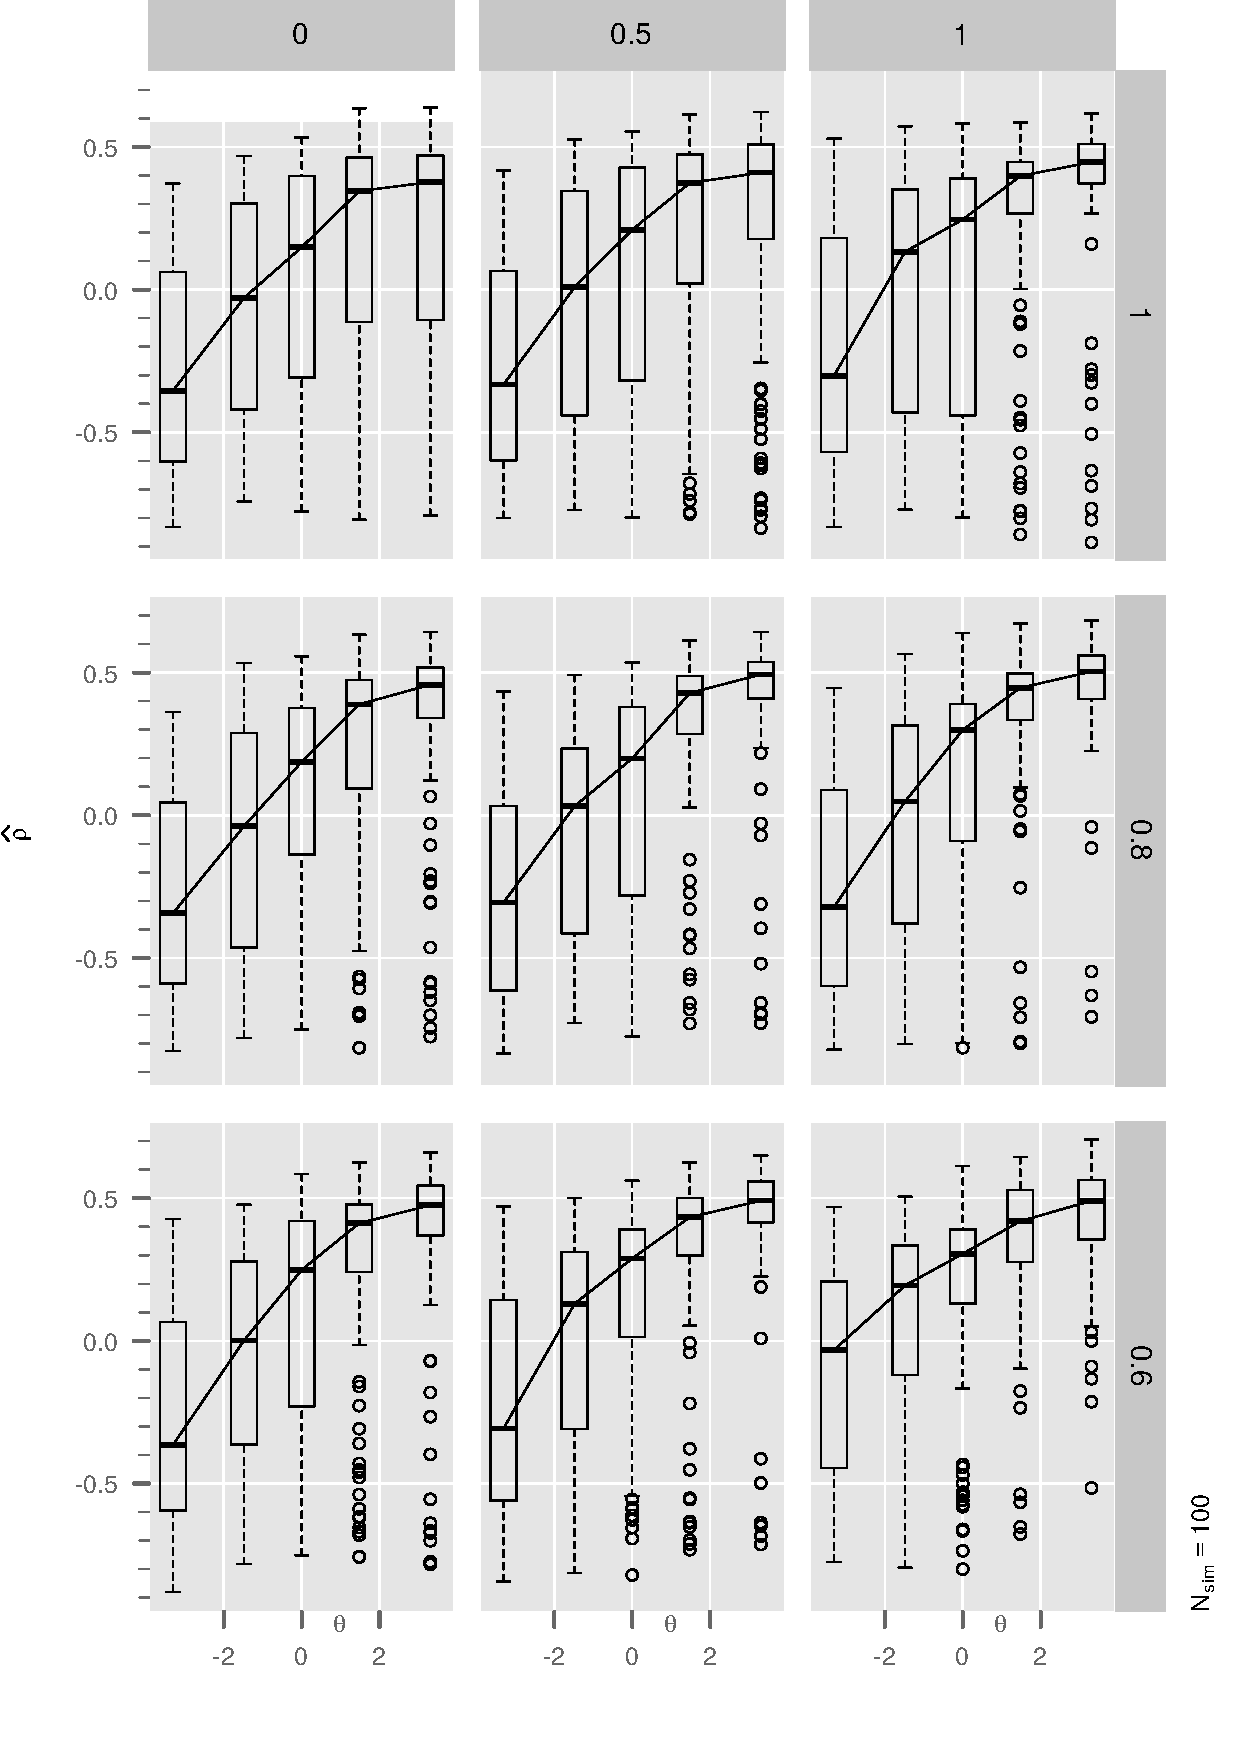
\includegraphics[width=1.00\textwidth]{Figure2/boxplotArray2.pdf}
\end{center}

\end{frame}

\hypertarget{robustness-to-non-normality}{%
\section{Robustness to
non-Normality}\label{robustness-to-non-normality}}

\begin{frame}{Frank copula}
\protect\hypertarget{frank-copula}{}

\begin{itemize}
\tightlist
\item
  we set standard Normal \emph{marginals}
\item
  association parameter, Frank \(\theta\)

  \begin{itemize}
  \tightlist
  \item
    \(\theta \rightarrow \tau \rightarrow \rho\)
  \end{itemize}
\item
  \emph{joint} distribution is \alert{non-} BVN
\end{itemize}

\end{frame}

\begin{frame}[fragile]

\begin{center}
  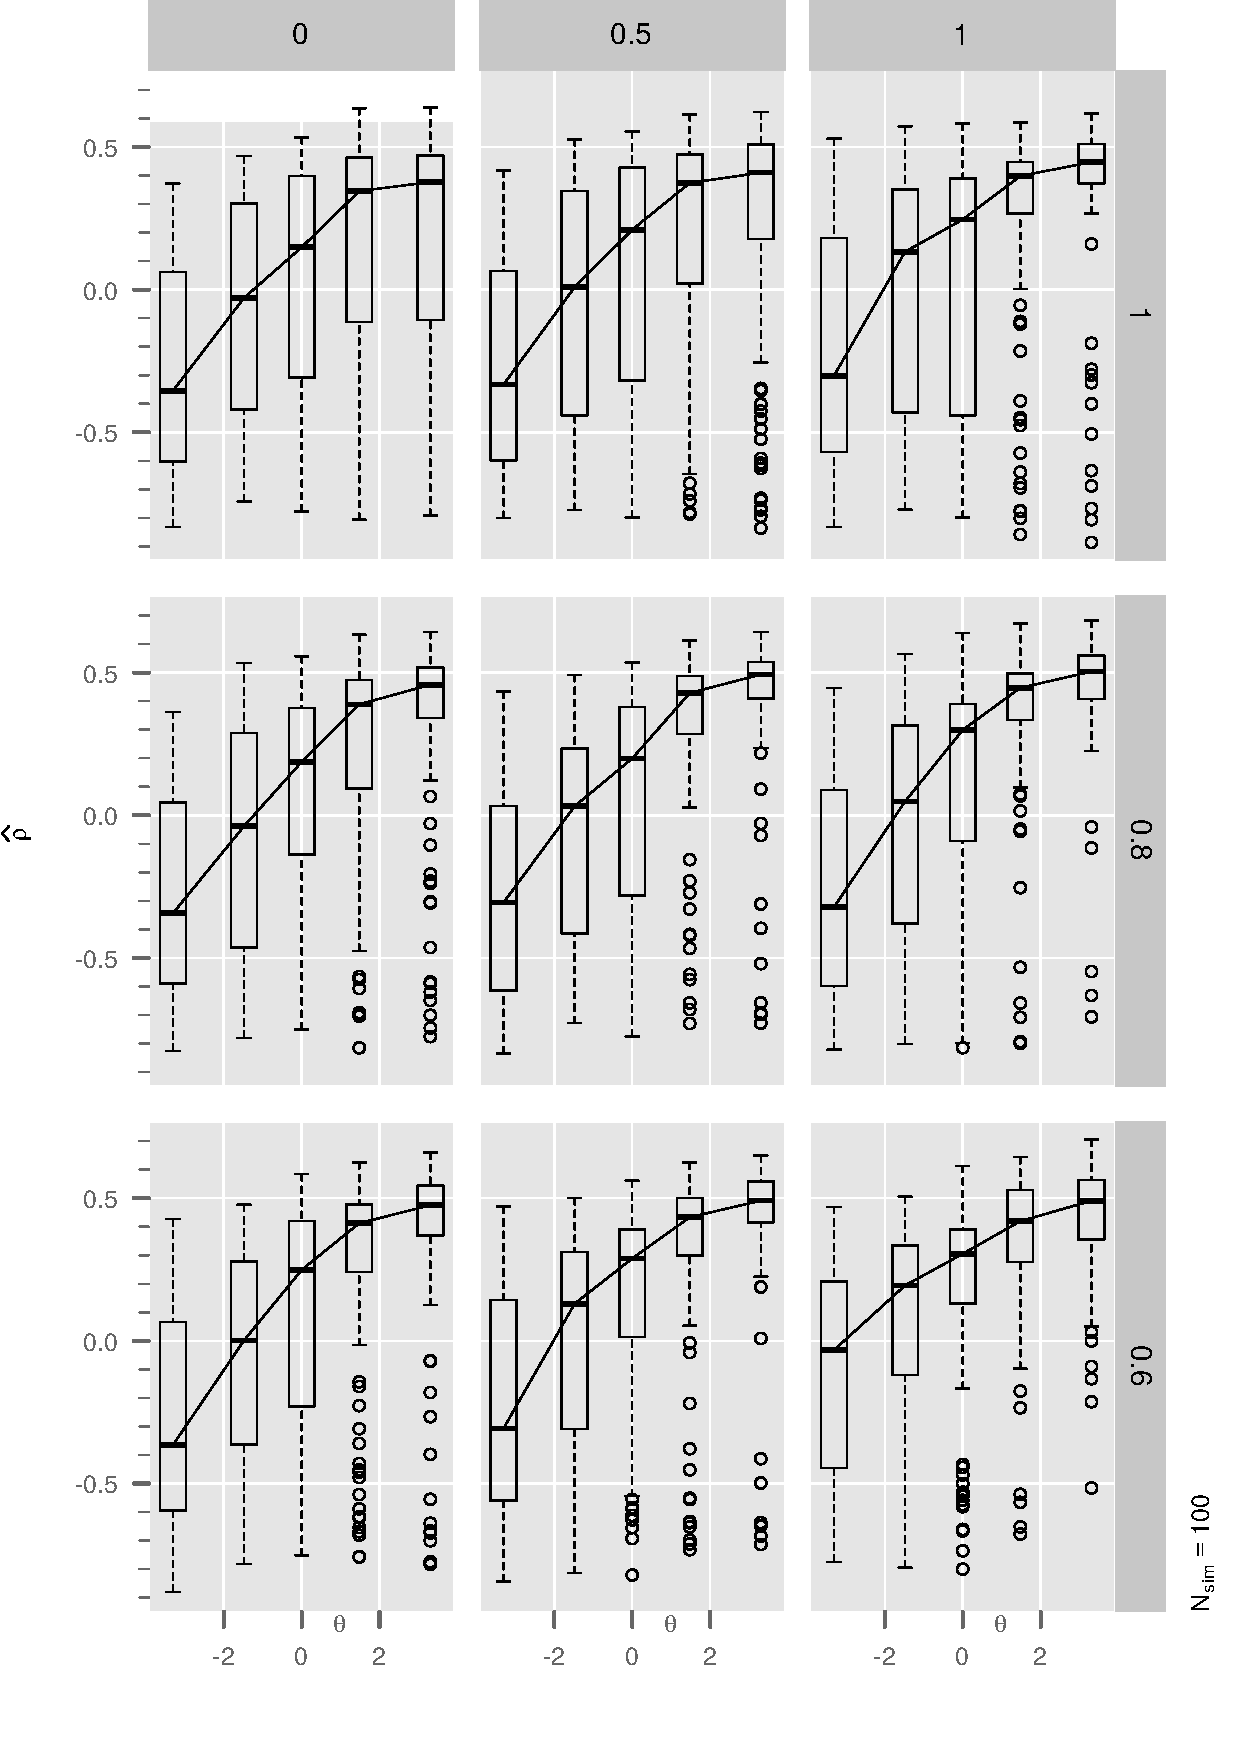
\includegraphics[width=1.00\textwidth]{Figure2/boxplotArray2.pdf}
\end{center}

\end{frame}